\input{pre}

\usepackage{csvsimple}
% \titleformat{\section}{\fontfamily{put}\selectfont}{\thesection}{1em}{}
 % \titleformat{\subsection}
    % {\normalfont\bf}{\thesection}{1em}{}
\usepackage{graphicx}
\usepackage{times}
% \usepackage{scrextend}
% \changefontsizes[9pt]{9pt}

\usepackage{datatool}



\title{Statistische Verfahren: \\ Projekt 4 - Nahinfrarotspektroskopie I}
\author{Tobias Giesemann \\ Ferdinand Rewicki \\ Moritz Preu\ss\@}
% \date{}
\newcommand{\email}{tobias.giesemann@uni-jena.de \\ ferdinand.rewicki@uni-jena.de \\ moritz.preuss@uni-jena.de}

\begin{document}
	\newgeometry{top=40mm,left=45mm,right=45mm}
	\onecolumn
	\maketitle
	\thispagestyle{empty}
	\hrule
	\medskip
	\begin{abstract}
		\itshape
		In der vorliegenden Arbeit wird eine Methode zur Ableitung einer Kalibierfunktion zur Bestimmung des Stickstoffgehalts in Bodenproben vorgestellt.
Basierend auf den zugrunde liegenden physikalischen und chemischen Eigenschaften der Nahinfrarotspektroskopie wird ein lineares Modell formuliert. 
Hierfür wurden potenzielle Prediktoren entsprechend ihrer Variabilität für das Maximalmodell ausgewählt und mit Hilfe von Mallow's $C_p$-Kriterium ein Idealmodell ermittelt. 
Darüber hinaus wurde der Einfluss des Stichprobenumfangs auf den durch den minimalen $C_p$-Wert geschätzten Vorhersagefehler untersucht.
	\end{abstract}
	\medskip
	\hrule
	\tableofcontents
	\newpage
	\null
	\thispagestyle{empty}
	\newpage
	\restoregeometry
	\pagenumbering{arabic}

	\linespread{1.1}\selectfont
	\twocolumn[
		{\begin{@twocolumnfalse}
			\thispagestyle{titlestyle}
			{\huge\bfseries \begin{center}{Statistische Verfahren: \\ Projekt 4.1 - Nahinfrarotspektroskopie I}\end{center}}
			\bigskip
			\begin{minipage}[t][][l]{0.33\textwidth}
				\centering{Tobias Giesemann \\ tobias.giesemann@uni-jena.de}
			\end{minipage}
			\hfill
			\begin{minipage}[t][][l]{0.33\textwidth}
				\centering{Ferdinand Rewicki \\ferdinand.rewicki@uni-jena.de}
			\end{minipage}
			\hfill
			\begin{minipage}[t][][l]{0.33\textwidth}
				\centering{Moritz Preu\ss\@ \\ moritz.preuss@uni-jena.de}
			\end{minipage}
			\bigskip
			\bigskip
			\hrule
			\medskip
			\begin{abstract}
				\itshape
				In der vorliegenden Arbeit wird eine Methode zur Ableitung einer Kalibierfunktion zur Bestimmung des Stickstoffgehalts in Bodenproben vorgestellt.
Basierend auf den zugrunde liegenden physikalischen und chemischen Eigenschaften der Nahinfrarotspektroskopie wird ein lineares Modell formuliert. 
Hierfür wurden potenzielle Prediktoren entsprechend ihrer Variabilität für das Maximalmodell ausgewählt und mit Hilfe von Mallow's $C_p$-Kriterium ein Idealmodell ermittelt. 
Darüber hinaus wurde der Einfluss des Stichprobenumfangs auf den durch den minimalen $C_p$-Wert geschätzten Vorhersagefehler untersucht.
			\end{abstract}
			\medskip
			\hrule
			\bigskip
			\bigskip
			\bigskip
		\end{@twocolumnfalse}}
	]

	\linespread{1.15}\selectfont
	
	%\thispagestyle{mainstyle}

	\section{Einleitung}
\label{sec:Einleitung}

    Die Zusammensetzung des Boden ist ein wesentlicher Faktor für einen ertragreichen und nachhaltigen Anbau von Pflanzen in der Landwirtschaft.
    Wichtige Parameter hierfür sind der organische Kohlenstoff des Bodens sowie der im Boden gebundene Stickstoff, durch deren Messung Fragen über die Fruchtbarkeit des Bodens, sowie Erkenntnisse über den Effekt der Bodennutzung beantwortet werden können.\cite{Poeplau2013}
    Die Messung der genannten Parameter ist durch sogenannte Fraktionierung der Bodenprobe möglich.
    Etablierte Messverfahren sind jedoch kostenintensiv, nicht vollständig standardisiert, und weisen eine schlechte Reproduzierbarkeit in verschiedenen Laboren auf.\cite{Poeplau2013}
    Aus diesem Grund sind Messverfahren notwendig, welche die zuverlässige und effiziente Ermittlung organischen Kohlenstoffs und gebundenen Stickstoffs des Bodens zulassen.
    Ein seit den sechziger Jahren vielfach eingesetztes Messverfahren ist die sogenannten Nahinfrarot Spektroskopie. \cite{Agelet2010}
    Diese erlaubt die Schätzung der aufwendig bestimmbaren Parameter N und SOC mit Hilfe der leicht messbaren Nahinfrarotspektren.
    Die Bestimmung und Validierung eines hierfür notwendigen Modelles für den Stickstoffgehalt in der Bodenprobe sind Gegenstand dieser Arbeit.

	
% section Einleitung
	\section{Hintergrund}
\label{sec:Hintergrund}
	
	\subsection{Gebundener Stickstoff}
	\label{ssec:Gebundener Stickstoff}
	
	Durch den sogenannten Stickstoffkreislauf geschieht der fortwährende  Austausch und die Umwandlung von Stickstoff.
	Der im Boden gebundenen Stickstoff ist ein unentbehrlicher Nährstoff für Pflanzen und Lebewesen.
    Zur Steigerung der Ernte ist der Einsatz von Stickstoffdünger daher gängige Praxis in der Landwirtschaft.(\textbf{Quelle...}
    Dies kann dann zu Problemen führen, wenn zu einer Übersättigung des Bodens mit Stickstoff kommt.
    Stickstoff liegt im Boden in Form von Ammonium ($NH_4^+$) und Nitrat ($NO_3^-$) vor.
    Durch das Ausschwemmen des für das Pflanzenwachstum wichtige Nitrat kann dieses in das Grundwasser gelangen, was durch in höherer Konzentration eine Gefahr für die Umwelt werden kann.
    Für den Erfolg der Landwirtschaft als auch für den Schutz der Umwelt ist daher eine zuverlässige und effiziente Ermittlung des Nitratgehalts im Bodens von entscheidender Bedeutung.
    Die Stoffmenge von Stickstoff ($N$) in einer gegebene Probe $P_i$ lässt sich wie folgt berechnen:
    	\[
			c_{(N)} \define \frac{n_{(N)}}{V_P}
		\]
    Für eine gegebene Stoffmengen der gesamten Probe $n_0$ definieren wir dann den Stoffmengenanteil von Stickstoff als,
        \[
			X_{(N)} \define \frac{c_{(N)}}{c_0} = \frac{n_{(N)}}{n_0}
		\]
   
	% subsection Gebundener Stickstoff

	\subsection{Nahinfrarotspektroskopie}
	\label{ssec:nirs}
	
		Bei der Nahinfrarot Spektroskopie kommen elektromagnetische Wellen im Bereich zwischen 120THz und 400 THz zum Einsatz. \cite{Agelet2010}
		Das Messverfahren nutzt die Tatsache, dass bei der Bestrahlung einer Probe mit Licht Teile des Lichts reflektiert, hindurch gelassen oder absorbiert werden.
		Von besonderem Interesse ist hierbei die Reflexion des Lichts.
		Dieses lässt in die zwei Komponenten Spiegelreflexion und diffuse Reflexion unterscheiden.
		Da die Teile des Lichts welche diffus reflektiert wurden tiefer in die Proben eindringen, können aus diesen Informationen gewonnen werden. 
		Für eine Wellenlänge $\lambda$ ist das relative Reflexionsvermögen $\delta(\lambda)$ definiert als:
		\[
			\func{\delta}{(0,\infty)}{(0,\infty)},\qquad \delta(\lambda) \define \frac{P_\m{r}(\lambda)}{P_s}
		\]
		
		wobei $P_\m{r}(\lambda)$ die Reflexion einer Probe und $P_0$ die Reflexion eines Material mit einer Reflexion nahe $100\%$ ist.
		
		Es lässt sich ein Zusammenhang zwischen dem relativen Reflexionsvermögen und der Absorption herstellen.
		Hierzu definieren wir die Absorption zunächst als:
		
		\[
			-\log \delta(\lambda) = -\log \frac{P_\m{r}(\lambda)}{P_s}
		\]
		
		Beers Law beschreibt den Zusammenhang zwischen der Konzentration einer Probe und deren Absorbtion bestimmter Wellenlänge.
		Eine direkte Messung des absorbierten Lichts ist nicht möglich, kann aber durch aber wie folgendermaßen mit relativen Reflexion in Verbindung gebracht werden.
		\[
			-\log \delta(\lambda) = \varepsilon(\lambda) c_i d
		\]
		,wobei 
		Summarizing, NIR measurements for analytical purposes
can be carried out in two modes: transmission or diffuse
reflection. Diffuse reflection mode allows working with thicker
and denser samples without inducing as much heating as trans-
mission. While sample path length is pre-determined and must
be kept constant for transmittance measurements, the minimum
sample required in reflectance mode is highly dependent on
the wavelength range used in the analysis and sample charac-
teristics such as density or packing, particle size, and material
		
		 
		
		of a 

	% subsection nirs

% section Hintergrund
	\thispagestyle{mainstyle}
	% !TeX spellcheck = de_DE
\section{Methodik}
\label{sec:Methodik}

	\subsection{Datensatz}
	\label{ssec:Datensatz}

	    Der für die Modellwahl verwendete Datensatz beinhaltet die logarithmierten relativen Reflexionswerte $-\delta(\lambda)$ bei Wellenlängen zwischen 1400 nm und 2672 nm in einem Abstand von 4 nm sowie die Stoffmengeanteile $y^{(N)}$, $y^{(SOC)}$ und entsprechenden pH-Werte von insgesamt 533 Proben.
	    Informationen über die chemische Zusammensetzung der Probe in den Reflexionswerten im Nahinfrarotbereich sind stark überlagert. \cite{Agelet2010}
	    Aus diesem Grund ist eine sorgfältige Auswahl relevanter Wellenlängen von besonderer Bedeutung für die Erstellung eines zuverlässigen Modells.


	% subsection Datensatz

	\subsection{Statistisches Modell}
	\label{ssec:Statistisches Modell}

	    Sei $n\in\SN$ die Größe des Datensatzes und $k\in\SN$ mit $k< n$ die Anzahl der Wellenlängen im Datensatz.
	    Entsprechend Abschnitt \ref{ssec:Datensatz} definieren wir dann die Einflussgröße $x_{ij}$ als für die $i$te Probe und $j$te Wellenlänge als
	    \[
			x_{ij} \define -\lg \delta_i(\lambda_j)
		\]
		für jedes $i,j\in\SN,i\leq n,j\leq k$.

	    Der Stoffmengenanteil des Stickstoffs  $y^{(N)}$ stellt die Zielgröße unseres späteren Modells dar.
	    Wie definieren hierfür den Vektor der Stoffmengenanteile $y_i$ der $i$ten Probe als den $n$-dimensionalen Vektor
		\[
			 y^{(N)} \define \curvb{y^\m{(N)}_i}
		\]

        Nachdem wir sowohl die Einflussgrößen als auch die Zielgröße für das lineare Modell definiert haben, lassen sich diese nun in Zusammenhang bringen.
        Es ist plausibel anzunehmen, sich die Zielgröße durch einen Linearkombination der Einflussgrößen beschreiben lässt.
        Hierfür definieren wir zunächst $Y^\m{(N)}$ als einen zufälligen Vektor von $y^\m{(N)}$ mit
        \[
			 \expect Y^\m{(N)} \define \beta_0 + \sum_{j=1}^k{x_{ij}\beta_j}
		\]

		Zudem ist es notwendig eine Variable $\varepsilon^\m{(N)}$ einzuführen welchen den Zufall der Messungen beschreibt.
	    In Matrixschreibweise lässt sich dies als die Designmatrix $\mathbb{X} \in \SR^{n \times (k+1)}$, dem Parametervektor $\beta \in \SR^{k+1}$ und dem stochastisch  verteilten Parameter $\varepsilon^\m{(N)}$ darstellen, sodass gilt,
		\[
			Y^\m{(N)} = \mathbb{X}\beta + \varepsilon^\m{(N)}
		\]
		mit
		\[
			\expect \varepsilon^\m{(N)} = 0, \qquad \cov \varepsilon^\m{(N)} = (\sigma^2)^\m{(N)} \idmat
		\]
		wobei $(\sigma^2)^\m{(N)} \in (0,\infty)$.
		Weiterhin soll angenommen werden, dass $\varepsilon^\m{(N)}$ normalverteilt ist mit
	    \[
			\varepsilon^\m{(N)} \sim \FN \curvb{0,(\sigma^2)^\m{(N)}\idmat}
		\]
	    sodass sich für das Gesamtmodell gilt
		\[
			Y^\m{(N)} \sim \FN \curvb{\mathbb{X}\beta^\m{(N)},(\sigma^2)^\m{(N)} \idmat}
		\]

	% subsection Statistisches Modell

	\subsection{Statistische Modellwahl im Falle von NIR-Spektroskopie}
	\label{ssec:mlr}
	Seien $Y\in \rm I\!R^{n}$ die Zielgröße eines statistischen Modellwahlverfahrens und $X \in \rm I\!R^{n \times d}$ die Matrix von $d$ Einflussparametern und $n$ Beobachtungen.
	Zur Wahl einer geeigneten Menge von Einflussparametern $x_i$ auf die Zielgröße $y_i$  wird im klassischen linearen Modell die Modellwahl über eine hierarchische Aufstellung von linearen Modellen erriecht.
	Beginnend mit dem minimalen Modelle $E(Y_i) = \beta_0$ werden dem Modell nach und nach neue potenzielle Einflussparameter $x_{ik}$ hinzugefügt.
	Zu jedem dieser neuen $x_{ik}$ wird dann eine Teststatistik aufgestellt, die darauf hinweist, ob der gewählte Parameter wichtig ist ist oder nicht.
	Dabei ist die Nullhypothese, dass $x_{ik}$ keinen Einfluss auf die Zielgröße hat: $ H_0 = \beta_k = 0$ und wird abgelehnt, falls $H_1 = \beta_k \neq 0$ zutrifft.
	Dies wird über die T-Teststatistik erreicht,  wobei für den Fall, dass $H_0$ richtig ist, gilt: $\frac{\hat{\beta_k}}{\sqrt{\sigma^2(X^TX)^{-1}_{kk}}} \sim t_{n-(k+1)}$.
	Mit diesem Modellwahlverfahren ergeben sich einige Schwierigkeiten, wobei die für unseren Fall besonders schwerwiegenden herausgehoben werden: In dieser Arbeit haben wir es mit einer großen Anzahl potenzieller Einflussvariablen auf dem Nah-Infrarotspekturm zu tun.
	A priori kann schwer eine inhaltliche Deutung vorgenommen werden, die gewisse Wellenlängen bevorzugt. Daher ist eine hierarchische Modellwahll mit wenigen, wohlüberlegten Einflussvariablen nicht möglich.
	Demnach muss in dieser Arbeit die Anzahl der möglichen Einflussgrößen stark erhöht werden und hier bekommen wir ein Problem mit der T-Teststatistik.
	Es ließen sich sehr viele unterschiedliche Kombinationen von Einflussgrößen aufstellen und in eine hierarchische Form bringen.
	Doch da wir bei der T-Teststatistik ein $\underline{zufälliges}$ Intervall konstruieren, gegen das unsere Hypothese getestet wird, ist die Wahrscheinlichkeit bei oft wiederholten Tests fälschlicherweise die Nullhypothese abzulehnen steigend mit Anzahl der Versuche.
	An ein automatisiertes Modellwahlverfahren, das in dieser Arbeit von Vorteil ist, ist also mittels des T-Tests nicht zu erreichen. (siehe Skript 11/2018)
	Stattdessen bietet sich eine Modellwahl basierend auf dem erwarteten Prognosefehler ("sum of prediction squared error", SPSE) an:
	\[
		SPSE \define \expect \sum_{i=1}^{n} (Y_{i+n} - x_{i}^\m{(M)}\hat{\beta_i}^\m{(M)})^2
	\]

	Hierbei sind die Werte in $Y_{i+n}$ neue, potenzielle Beobachtungen zum Einflussvektor $x_i$ und $x_{i}^{(M)}\hat{\beta_i}^{((M)}$ ist sind die Prognosewerte aus dem Modell $M$.
	Der Prognosefehler lässt sich in 3 Terme zerlegen: Einen irreduzierbaren Prognosefehler, der unabhängig von dem momentan betrachteten Modell ist, einen Biasterm, der die Abweichung des aktuellen Modells $M$ vom Prognosemodell als Summe der quadrierten Prognose-Verzerrungen anzeigt und einen Varianzterm, der die Ungenauigkeiten widerspiegelt, die sich aus der Schätzung von $(|M|+1)$ unbekannten Parametern ergibt.
	Der SPSE lässt sich über unterschiedliche Wege berechnen / abschätzen, mithilfe neuer Beobachtungen (1), (wiederholter) Zerlegung der Ursprungsdaten in Test- und Trainingsdaten (2) oder mittels Schätzung basierend auf der Residuenquadratsumme ("residual squared sum", RSS), hier im Vergleich zu o.g. SPSE:

	\[
	\expect RSS^\m{(M)} \define \sum_{i=1}^{n} \expect (Y_{i} - \hat{Y_i}^\m{(M)})^2
	\]
	\[
	SPSE^\m{(M)} \define \sum_{i=1}^{n} \expect (Y_{i+n} - \hat{Y_i}^\m{(M)})^2
	\]

	Es kann gezeigt werden, dass RSS den Wert von SPSE systematisch unterschätzt, dass diese Unterschätzung jedoch behoben werden kann (siehe Skript 12/2018):

    \[
	SPSE^\m{(M)} \define \expect RSS^\m{(M)} + 2\tilde{\sigma}_{\underline{full}}^2(|M|+1)
    \]

    wobei $\tilde{\sigma}_{full}^2$ die Varianz des größten Modells ist.

	% subsection mlr

	\subsection{Mallow's $C_{p}$}
	\label{ssec:mallows-C_p}



	\subsection{Model Validation}
	\label{ssec:model-validation}
    Ein geeigneter Parameter zur Messung der globalen Anpassungsgüte einer Regression ist $R^2$. \textbf{Quelle}
    \[
    {R^2}^{(M)} \define \frac {\sum_{i=1}^n \curvb{\hat{y}^{(M)}_i - \overline{y}}^2}{\sum_{i=1}^n \curvb{y_i - \overline{y}}^2}
    \]
    Dieser beschreibt den Anteil der durch die Regression erklärten Quadratsumme an der totale Quadratsumme und nimmt dadurch Werte zwischen 0 und 1 an.
    Während ein $R^2$ von 1 für einen perfekten linearen Zusammenhang steht bedeutet ein Wert von 0, dass kein linearer Zusammenhang vorliegt.
    Für das gewählte Modell ergibt sich ein Wert von \textbf{....}.
    Dies weißt auf eine relativ gute Anpassung durch das gewählte Modell hin. \textbf{zu prüfen}
    Zudem ist es sinnvoll neben dem Parameter $R^2$ ein Korrelationsdiagramm zwischen der durch das Modell geschätzten Ausprägung $\hat{y}_i$ und dem wahren Wert $y_i$ zu betrachten.
    \textbf{Einfügen von Grafik: Korrelationsdiagramm}
    
    


	% subsection model-validation

	\subsection{Assessment by Simulation}
	\label{ssec:simulation}



	% subsection simulation
% section methodology

	\section{Implementation}
\label{sec:implementation}
	
	\subsection{Choosing a Neighbour}
	\label{ssec:choosing-a-neighbour}
		
		We stated in section \ref{ssec:model-selec} that we want to select a \enquote{good} model for the prediction.
		
	% subsection choosing-a-neighbour
		
	\subsection{Additional Functions}
	\label{ssec:add-func}
	
		All other functions were defined following a standard scheme.
		It follows from \ref{ssec:mallows-C_p} that
		\[
			\m{cost}(M)\define C_\m{p}^{(M)}
		\]
		
	%subsection Additional Functions
	
		
% section implementation
	\section{Ergebnisse und Diskussion}
\label{sec:discuss}

\subsection{Modellwahl}
\label{ssec:discuss:modelselect}
Unter Anwendung der in Abschnitt \ref{ssec:modellselektion} bzw \ref{ssec:impl:modelwahl} vorgestellten Methode wurde aus einem 149 Prädiktoren umfassenden Maximalmodell das in Tabelle \ref{table:model_parameters} angegebene, 50 Prädiktoren große Modell anhand des kleinsten $C_p$-Wertes von $\m{\approx3.92}$ als optimales Modell ausgewählt.\\
\begin{figure*}[ht]
    \centering
    \begin{tikzpicture}
        \begin{axis}[ 
            ylabel = $N_{origin}$,
            xlabel = $N_{est}$,
            xmin=0, xmax=0.8,
            ymin=0, ymax=0.8,
            legend pos = north west,
            scaled ticks = false,
            width = .5\textwidth,
            ymajorgrids,
            xmajorgrids,
            %height = 8cm,
            cycle list name=black white
        ]
            \addplot +[only marks]
            table[x=origN, y=simN, col sep=comma] {plots/data/correlation_plot_data.csv};
            %\addlegendentry{{\scriptsize Variablität}}
            \begin{scope}[red]
                \draw[red] ({axis cs:0,0}) -- ({axis cs:1,1});
            \end{scope}   
            %\addplot +[ycomb, no marks, dashed] 
            %table[x=x, y expr=0.0105 ,col sep=comma] {plots/data/selectedFeatures.csv};
            
            
        \end{axis}
    \end{tikzpicture}
    \captionof{figure}{Korrelationsplot}
    \label{fig:correlation}
\end{figure*}
Der Wert des Bestimmtheitsmaßes $R^2 = 0.82$ zeigt, dass das gewählte Modell die Varianz in den Daten gut erklären kann. Dies spiegelt auch das in Abbildung \ref{fig:correlation} abgebildete Korrelationsdiagramm wieder, in welchem der wahre Wert auf der x-Achse und der geschätzte Stickstoffmengenanteil auf der y-Achse aufgetragen sind.
Abweichungen sind lediglich im oberen Bereich ab $0.3$ zu beobachten, wo der Stoffmengenanteil des Stickstoffs durch das Modell unterschätzt wird.
Dies lässt dich vermutlich durch die geringe Datendichte in diesen Bereichen erklären.
Insgesamt kann man sagen, dass die bisherigen Untersuchungen auf ausreichend gute Prognosen durch das Modell hindeuten.

\begin{figure}[H]
    \centering
    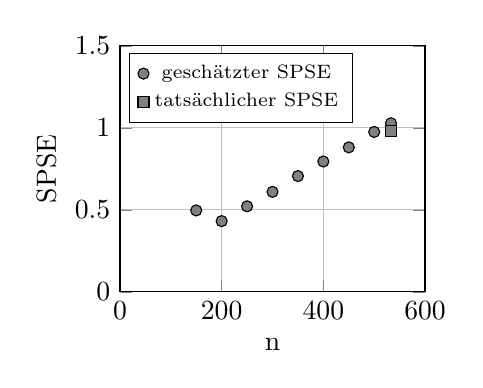
\begin{tikzpicture}
        \begin{axis}[ 
            ylabel = SPSE,
            xlabel = n,
            xmin=0, xmax=600,
            ymin=0, ymax=1.5,
            legend pos = north west,
            scaled ticks = false,
            width = .45\textwidth,
            ymajorgrids,
            xmajorgrids,
            %height = 8cm,
            cycle list name=black white
        ]
            \addplot +[only marks]
            coordinates {
                (150,0.4964226)
                (200,0.4312206)
                (250,0.5213190)
                (300,0.6097658)
                (350,0.7058959)
                (400,0.7947748)
                (450,0.8807918)
                (500,0.9750933)
                (533,1.0280917)
            };
            \addlegendentry{{\scriptsize geschätzter SPSE}}
            
            \addplot +[only marks]
            coordinates {
                (533,0.9813258)
            };
            \addlegendentry{{\scriptsize tatsächlicher SPSE}}
        \end{axis}
    \end{tikzpicture}
    \captionof{figure}{geschätzer sowie tatsächlicher SPSE in Abhängigkeit der Stichprobengröße}
    \label{fig:spse}
\end{figure}

\subsection{Simulation}
\label{ssec:discuss:simulation}
Die vorliegende Arbeit sollte den Einfluss des Stichprobenumfangs auf die SPSE-Schätzung mithilfe Mallow's $C_p$ untersuchen. Die hier angegebenen Werte spiegeln den Mittelwert aus 10 Durchläufen wieder.

\begin{table}[!h]
    \centering
	\begin{tabular}{|l|l|}
		\cline{1-2}
		$n$   & $\hat{SPSE}$ \\ 		\cline{1-2}
		150 &  0.4964226   \\ \cline{1-2}
		200 &  0.4312206   \\ \cline{1-2}
		250 &  0.521319    \\ \cline{1-2}
		300 &  0.6097658  \\ \cline{1-2}
		350 &  0.7058959   \\ \cline{1-2}
		400 &  0.7947748 \\ \cline{1-2}
		450 &  0.8807918  \\ \cline{1-2}
		500 &  0.9750933   \\ \cline{1-2}
		533 &  1.028092   \\ \cline{1-2}

	\end{tabular}
	\caption{Über Mallow's $C_p$ geschätzte SPSE Werte mit zugehörigen $n$}
\end{table}

Wie in Abbildung \ref{fig:spse} zu erkennen ist steigt der geschätzte SPSE-Wert außer bei $n < 200$ monoton und nahezu linear mit zunehmender Stichprobengröße. Dies lässt auf einen starken linearen Einfluss von $n$ auf den SPSE schließen. In der Berechnung des SPSE ist $n$ sowohl als Faktor im unkontrollierten Prognosefehler als auch im Biasterm vorhanden, was den Einfluss auf das Ergebnis bereits vermuten ließ.
Der tatsächliche SPSE von 0,981 wird bei der Schätzung über Mallow's $C_p$ mit derselben Stichprobengröße (533) um knapp 5\% überschätzt und liegt bei 1,028. 
Daraus lässt sich schließen, dass der Biasterm durch die zufällige Simulation wohl leicht überschätzt wurde.
Wir können also schlussfolgern, dass SPSE Werte, die auf verschiedenen Stichprobengrößen beruhen, normiert werden müssen, um miteinander vergleichbar zu sein.

Eine Schlussfolgerung aus den hier vorgefundenen Werten ist nun, dass SPSE Werte zur Vergleichbarkeit mittels des Stichprobenumfangs genormt sein müssen, um miteinander vergleichbar zu sein.
	%\section{Simulation}
\label{sec:simulation}
	
	...of table \ref{tab:sim-res}.
		
	\input{sec/simulation-table}
	
	

% section simulation
	\section{Conclusion}
\label{sec:conclusion}

	Using Mallow's $C_\m{p}$ criterion, we calibrated three predictive models for the soil parameters $p^{(\m{SOC})}$, $p^{(\m{N})}$ and $\m{pH}$.
	To construct ...
	

% section conclusion
	
	\bibliography{ref}
	
	\appendix
	\onecolumn
	\pagenumbering{roman}
	\section{Einflussgrößen und Parameter des Modells}
\label{sec:parameters}

\begin{table}[H]
	\center
    \begin{tabular}{rr|rr|rr|rr|rr}%
        $x_i$ & $\beta_i$ & $x_i$ & $\beta_i$ & $x_i$ & $\beta_i$ & $x_i$ & $\beta_i$ & $x_i$ & $\beta_i$
        \csvreader{tables/data/parameters.csv}{}
        {\\\hline\csvcoli & \csvcolii & \csvcoliii & \csvcoliv & \csvcolv & \csvcolvi & \csvcolvii & \csvcolviii & \csvcolix & \csvcolx }
    \end{tabular}
    \caption{Enthaltene Features und geschätzte Parameter $\beta$ des ausgewählten Modells}
	\label{table:model_parameters}
\end{table}
	\section{R Source Code}
\label{sec:r-source-code}

\lstinputlisting[basicstyle=\footnotesize\ttfamily, frame=single]{code/modelselect.R}
\clearpage
\lstinputlisting[basicstyle=\footnotesize\ttfamily, frame=single]{code/simulation.R}
\clearpage
\lstinputlisting[basicstyle=\footnotesize\ttfamily, frame=single]{code/helper.R}
\lstinputlisting[basicstyle=\footnotesize\ttfamily, frame=single]{code/spse.R}
\clearpage
\lstinputlisting[basicstyle=\footnotesize\ttfamily, frame=single]{code/main.R}


% section r-source-code
	
	\newpage
\thispagestyle{empty}
\section*{Statutory Declaration}
\bigskip

% contains the statutory declaration in accordance with German requirements on written examination to obtain an academic degree

We herewith declare that ...

\vspace{1 cm}

\noindent
Jena, 25th of August 2016

\vspace{1 cm}
\hspace{6 cm} Kazimir Menzel \hspace{3 cm} Markus Pawellek


\end{document}
